\documentclass[10pt]{article}

\usepackage[letterpaper,left=0.5in,right=0.5in,top=1in,bottom=1in]{geometry}

\usepackage[T1]{fontenc}
\usepackage[utf8]{inputenc}
\usepackage{lmodern}

\usepackage[activate={true,nocompatibility},final,tracking=true,kerning=true,spacing=true,factor=1100,stretch=10,shrink=10]{microtype}
\microtypecontext{spacing=nonfrench}
\usepackage{xspace}
\usepackage{amssymb,amsfonts,amsmath}
\usepackage{lipsum,xcolor}
\usepackage{graphicx}
\usepackage{float,caption,subcaption,wrapfig}
\usepackage{tcolorbox}
\usepackage{listings}
\usepackage{courier}
\usepackage[english]{babel}
\usepackage{textcomp}
\usepackage{csquotes}
\usepackage{siunitx}
\usepackage[makeroom]{cancel}
\usepackage[shortlabels]{enumitem}
\sisetup{mode=text,
         group-separator={,},
         detect-all,
         binary-units,
         list-units = single,
         range-units = single,
         range-phrase = --,
         per-mode = symbol-or-fraction,
         list-final-separator = {, and }
}

\lstset{basicstyle=\ttfamily,
        breaklines=true,
        numbersep=-8pt,
        numberstyle=\small,
        numbers=right,
        frame = single, 
        showstringspaces=false,    
        keywordstyle=\color{blue}\bf,
        commentstyle=\color{darkgray},
        stringstyle=\color{purple}\bf,
  }

\DeclareSIUnit\atm{atm}
\DeclareSIUnit\bar{bar}

\headheight = 13.6pt
\usepackage{fancyhdr}
\pagestyle{fancy}

\lhead{PH 641 Sp2020}
\chead{Quiz 12}
\rhead{Due 5:00 pm, 12 May 2020}

\rfoot{Submitted by: Paige Lorson}
\tcbset{width=(\linewidth-2mm),before=,after=\hfill,colframe=black,colback=white,}
\newcommand{\volume}{{\ooalign{\hfil$\vol$\hfil\cr\kern0.08em--\hfil\cr}}}
\newenvironment{Solution}
    {\textbf{Solution:}
    
    \vspace{5mm}
    \begin{tcolorbox}
    }
    {
    \end{tcolorbox}
    \vspace{5mm}
    % \newpage
    }
\newcommand{\vol}{{\ooalign{\hfil$V$\hfil\cr\kern0.08em--\hfil\cr}}}
\renewcommand\labelitemi{$\cdot$}

\begin{document}

\noindent\textbf{Quiz problem 1:} A continuous random variable $x$ has an associated probability distribution
\[
p(x)=\frac{\lambda}{2} \exp (-\lambda|x|)
\]

\begin{enumerate}

    \item Plot $p(x)$ and determine all allowed value(s) for $\lambda$


\begin{Solution}
\centering{
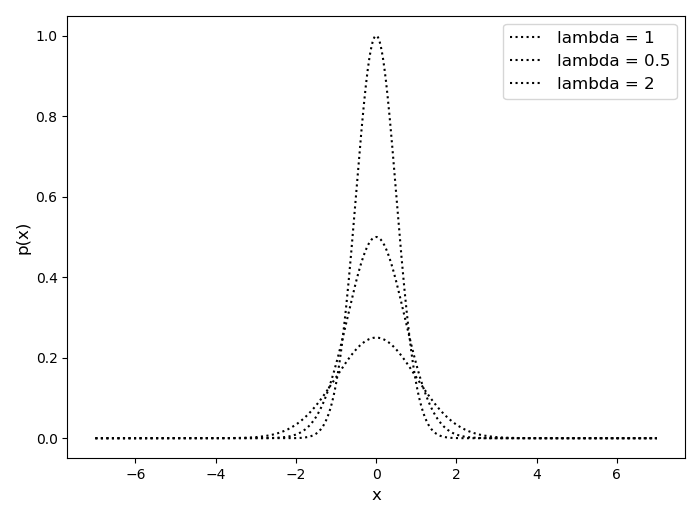
\includegraphics[width=4in]{Quizzes/plot_q12a.png}}
\end{Solution}

    \item A function $F(x)=x^{2}$ defines a new random variable $f=F(x)$. Calculate and write down $p_{F}(f) .$ Plot $p_{F}(f)$
Reminders:
i) $|x|=:$ absolute value of $x$
ii) $p_{F}(f)=\sum_{i} p\left(x_{i}\right)\left|\frac{d x}{d F}\right|_{x=x_{i}}$ Multiple values of $x$ can map onto one value of $f$
iii) In b) the new random variable is $f .$ You are calculating and plotting $p(f),$ there should be no more $x$ in your answer.

\begin{Solution}
\centering{
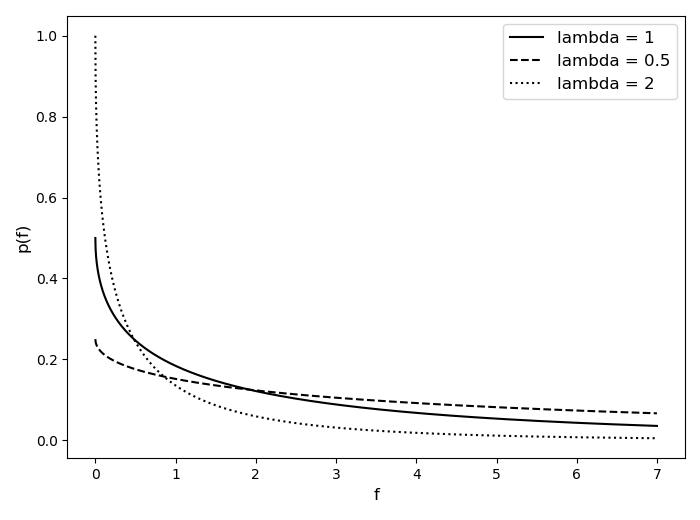
\includegraphics[width=4in]{Quizzes/plot_q12b.png}}
\end{Solution}
\end{enumerate}

\end{document}